Here we describe a few different kinds of random number generators, the math that makes them work, give examples of each kind, and give their strengths and weaknesses.

\subsection{Linear Congruential Generators}
\label{sec:lcg}
The Linear Congruential class of RNGs, or LCG for short, is a very old and relatively simple random number generator. They are based on the formula for a line, modulo another number. The following recurrence relation defines the LCG.
\begin{equation} \label{eq:lcg}
    X_{n+1} = (aX_n + c) \mod m
\end{equation}
Where the parameters are chosen with the following restraints:
\begin{align*}
    m,   \qquad & 0 < m \\
    a,   \qquad & 0 < a < m \\
    c,   \qquad & 0 \leq c < m \\
    X_0, \qquad & 0 \leq X_0 < m
\end{align*}
If $c = 0$, this particular class of of RNG is called a Lehmer, or Park-Miller RNG \cite{Payne:1969:CLP:362848.362860,Park:1988:RNG:63039.63042}.

The period of such generators depends heavily on the chosen parameters. It can be at most $m$, and as a result, $m$ is often chosen to be the largest number which can fit in the number of bits of the output; usually $2^{32}$ or $2^{64}$. Some common parameter sets in use include MINSTD, and glibc. A set of parameters notoriously deemed unfit for use is called RANDU, and is discussed below. Values for these parameters can be found in Table~\ref{tab:lcg_params}.

\begin{table}[tb]
    \caption{Table of common LCG parameters.}
    \label{tab:lcg_params}
    \begin{center}
        \begin{tabular}{l|ccc}
        \hline
        \hline
        \textbf{Name} & $m$ & $a$ & $c$ \\
        \hline
            MINSTD & $2^{32} - 1$ & 48271 & 0 \\
            glibc & $2^{31}$ & 1103515245 & 12345 \\
            RANDU & $2^{31}$ & 65539 & 0 \\
        \hline
        \hline
        \end{tabular}
    \end{center}
\end{table}

\subsubsection{Strengths}
LCG generators are tiny. They store a single word of state, are easy to seed, and with proper parameter choosing can be quite effective RNGs. However, some of the flaws greatly outweigh the lightweight and speed benefits of LCGs for all but the most basic of platforms, discussed next.

\subsubsection{Weaknesses}

LCGs have a fatal flaw, that is amplified by bad parameter choosing: their outputs fall in easily identifiable planes, as proved by Marsaglia \cite{randomnumbersinplanes}. This is most easily demonstrated by viewing the output of a notoriously bad set of parameters: RANDU. In Figure~\ref{fig:randu_fig}, the output of RANDU is treated as $(x,y,z)$ pairs as it is generated, then these points are plotted. It is obvious that all of the output falls in the same set of planes, and is not even an approximation of a truly random number generator. Better parameter choices alleviate this phenomenon by adding the number of planes that would come up in a test like this, and making them closer together, but the basic problem is unavoidable.

Another issue is the period length; at most the period length is $m$, which cannot be easily increased without increasing the number of bits in the word being operated on, which is not practical on modern architectures. In fact, experts recommend not even considering generators with periods $<2^{50}$ for anything but the most trivial uses \cite{L'Ecuyer:1992:TRN:167293.167354}.

\begin{figure}[tb]
    \begin{center}
        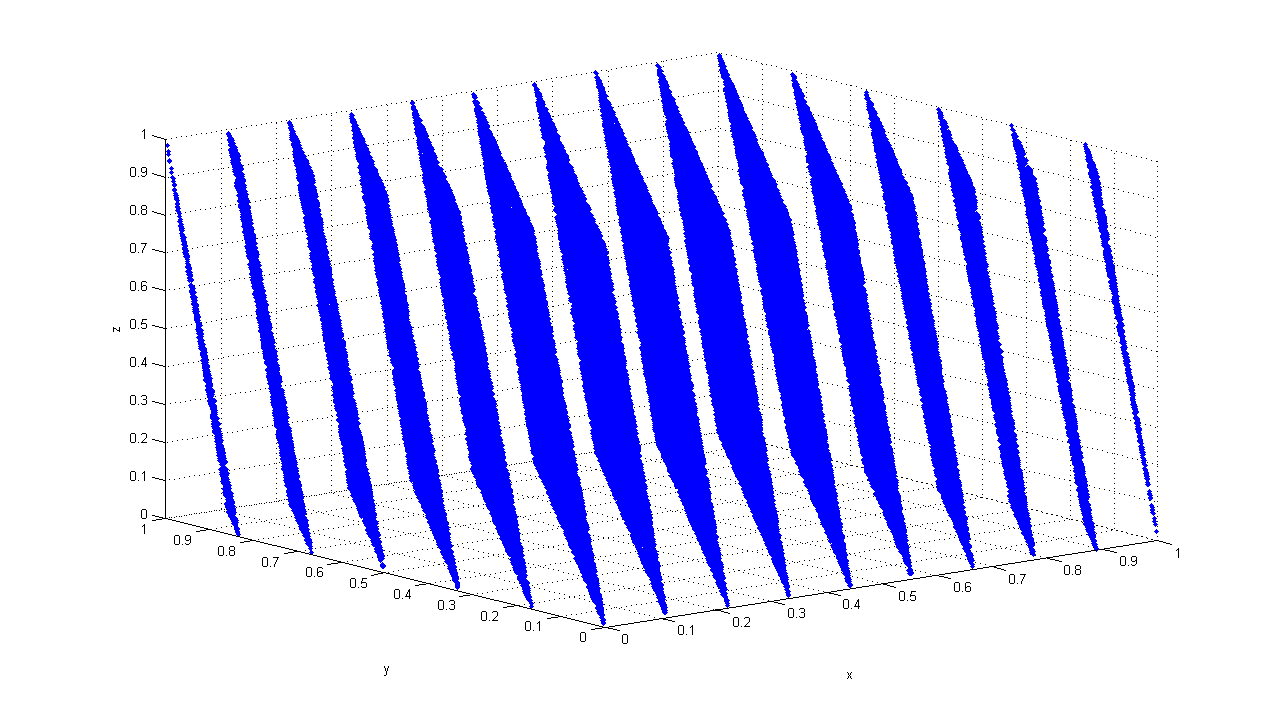
\includegraphics[width=\linewidth]{figures/randu.png}
    \end{center}
    \caption{The problem with LCGs demonstrated by RANDU; a MATLAB plot of consecutive outputs from RANDU used as $(x,y,z)$ points and plotted \cite{randu_fig}.}
    \label{fig:randu_fig}
\end{figure}

Despite these flaws, these extremely small and fast RNGs may still be suited to small embedded architectures and applications where speed is significantly more important than quality.


\subsection{Xorshift Generators}
\label{sec:xorshift}
A far more attractive choice than LCGs for those trying to implement RNGs with a lot of memory constraints, speed requirements, or a combination of the two on an embedded platform, is the Xorshift generator. Discovered and described by George Marsaglia \cite{marsaglia2003xorshift}, they are significantly more adept at creating sufficiently long periods for more applications.

Xorshift RNGs work by keeping a small amount of state (in many example implementations, four numbers), then repeatedly XORing these numbers with shifted versions of themselves. By doing this, the period of the generation can be $2^{32 * 4} = 2^{128}$ with very little code. The following is a short example for how easily Xorshift generators can be implemented. Let \texttt{t}, \texttt{x}, \texttt{y}, and \texttt{w} be seed values. Then, let \texttt{a}, \texttt{b}, and \texttt{c} be the parameters of the RNG. Then, the C style code is as simple as the following:

\begin{lstlisting}[frame=single,language=C++,basicstyle=\ttfamily]
// Random seed numbers
uint32_t t, x, y, w;
// Fixed constants for shifting
const uint32_t a, b, c;
uint32_t get_rand(void){
    t = x ^ (x << a);
    x = y;
    y = z;
    z = w;
    w = w ^ (x >> b) ^ t ^ t( >> c);
    return w;
}
\end{lstlisting}

Picking parameters for the directions and amounts to shift each state variable by is also relatively easy, and is discussed in \cite{marsaglia2003xorshift}, along with every set of appropriate parameters $a$, $b$, and $c$ for 32 bit and 64 bit words.

\subsubsection{Strengths}

Xorshift RNGs are very fast on modern architectures, and use very little state. They have longer periods than LCGs, and are easier to choose parameters for. These RNGs also perform far better on the Dieharder tests than LCGs, and pass the majority of them rather convincingly.

\subsubsection{Weaknesses}

However, the periods of Xorshift generators are not as large as some other generators. They are suitable for most uses, but in large simulations and Monte Carlo analysis, where massive amounts of random numbers are needed, the relatively small period could affect results.


\subsection{Lagged Fibonacci Generators}
\label{sec:laggedfib}
This section will describe Lagged Fib Generators.
\url{http://en.wikipedia.org/wiki/Lagged_Fibonacci_generator}
Also Mention Subtract with Carry:
\url{http://en.wikipedia.org/wiki/Subtract_with_carry}


\subsection{Mersenne Twister Generators}
\label{sec:mt}
One of the most commonly used RNGs, the Mersenne Twister (MT), was originally discovered by [?]. It is essentially an extension on top of the classical linear feedback shift register (LFSR). A simple LFSR is comprised of a bitwise shift-register where its input is determined by some combination of its current contents, traditionally the XOR of a select few bits from the register. While the LFSR is itself a RNG, its linear nature makes it very easily predictable. The Mersenne Twister improves upon the base concept by obfuscating the internal state of the register before feeding it into the XOR operation as well as applying additional transformations on the output to make the resulting sequence more uniform.

Mathematically, the MT operation for determining the next number in the sequence is:
\begin{equation} \label{eq:mt}
    X_{k+n} = X_{k+m} \oplus (X_k^u | X_{k+1}^ll)A
\end{equation}
Where $w$ is width of each word, $X_k^u$ is the upper $w-r$ bits of the $k$th word, $X_{k+1}^ll$ is the lower $r$ bits of the $k+1$th word, and $A$ is matrix of the form:
\[ \left( \begin{array}{ccc}
0 & I_{w-1} \\
a_{w-1} & {a_w ... a_0} \end{array} \right)\]
Colloquially, this is a matrix where the bottom row is a vector $a$ and the upper rows are comprised of a single identity matrix shifted to the right by one column. In effect, left multiplying by this matrix yields a vector whose bits are masked by $a$ and right shifted once. Again, this is similar to the operation of a simple LFSR except that the inputs to the XOR are masked before being processed.

Finally, to generate the desired random numbers, the sequence built from the above equations are transformed once more as such:
\begin{equation} \label{eq:mt_t1}
    y := x \oplus (x >> u)
\end{equation}
\begin{equation} \label{eq:mt_t2}
    y := y \oplus ((y << s) \cdot b)
\end{equation}
\begin{equation} \label{eq:mt_t3}
    y := y \oplus ((y << t) \cdot c)
\end{equation}
\begin{equation} \label{eq:mt_t4}
    y := y \oplus (y >> l)
\end{equation}
This is done so that each possible word occurs the same number of times within one period, with the exception of the all-zero word, which is less represented due to the underlying LFSR backbone.

The vast amount of parameters needed to define an instance of the MT algorithm along with the option of additional flexibility means that there exist many variants of this generator. For example, the 32-bit generator used in C++11 (MT19937) uses the following parameters: $w$=32, $n$=624, $m$=397, $a$=0x9908B0DF, $b$=0x9D2C5680, $c$=0xEFC60000, $u$=11, $s$=7, $t$=15, $l$=18.

\subsubsection{Strengths}
Mercenne Twister generators were originally designed to address concerns regarding the quality of randomness provided by prior generators. It is unsurprising then that these generators generally perform very well in the Dieharder tests. They are also well-known for their incredibly long periods ($2^{19937}-1$). Due to the popularity of this general type of generator, a number of specialized variants have also been created to mitigate its shortcomings, such as TinyMT, which boasts a miniscule internal state of only 127 bits. Of course, such variants do not come without drawbacks. In the case of TinyMT, shrinking the internal state size also necessarily decreases the length of the period. Still, this type of flexibility means that it is possible to gain the benefits of the MT generator tailored to the resource limits and constraints of specific applications, providing a great deal of versatility to the algorithm.

\subsubsection{Weaknesses}
The complex design of this generator unfortunately leads to slower performance, although it is certainly not the slowest of the bunch. Also, much like Lagged Fibonacci generators, MT generators store a great deal of state. This is especially true for MT generators since its implementations typically require much more state storage than its Lagged Fibonacci counterparts. Similarly, care must be taken when initializing the generator upon seeding. For example, large numbers of 0s in the initialization vector can cause the algorithm to produce long series of 0s as output until the internal recurrence breaks out of this pattern. It's also worth mentioning that despite its high quality outputs, the base MT algorithm does not pass the next bit test and is not suited for strict cryptographic applications.

